\subsection{Introduction}
Generally, it can be affirmed that different parts of the brain are responsible
for different actions and respond to different sensory inputs. It is
thought to be the most complex organ of the body and it consumes more or less
\(20\%\) of the overall ATP produced.\\
Let's see some characteristics of the \textbf{cerebral cortex}:
\begin{itemize}
    \item It is made of approximately \(14-16\) billions neurons.
    \item These neurons form about \(20\) trillions synapses.
    \item It is not a homogeneous tissue, due to the presence of layers with
          different properties.
    \item Pyramidal cells are particular excitatory neurons which exhibit the longest
          axons and big cell bodies.
\end{itemize}
It is important to point out that the brain is highly redundant:
just few regions are highly specialized, making easier to recover from injuries
thanks to brain plasticity.\\
The brain can be studied at several distinct scales, according to the recording site
and the number of recorded neurons producing a certain electrical signal. In general,
it can be stated that different neurons will respond to stimuli in different ways.\\
As said above, the cortex is structured in multiple layers, each of them with its own
properties, such as the density of neurons. Generally, deeper layers neurons
tend to project axons towards the surface, while upper layers cells project axons
mostly horizontally. As a result, the recorded activity is greatly variable according
to the selected recording site. In addition, also the signal-to-noise ratio (SNR) is
highly influenced by the location of the recording site, since it increses with the
distance from the source.

\subsection{Local Field Potential}
The \textbf{Local Field Potential (LFP)} refers to the electric potential measured in the
extracellular space around neurons. Its acquisition requires invasive electrodes
implanted into the brain of the subject, thus it has nothing to do with EEG. If compared to
spike recording, here the electrode is not inside or extremely close to a single neuron,
therefore the signal travels through the extracellular space according to Maxwell's
equations. The \textit{local} term is misleading, as it is meant to indicate that
the LFP is derived from a small number of sources: the action potential fired by a
neuron is highly attenuated by the extracellular space, thus the electrode can record
potentials in a limited radius. Nonetheless, the LFP signal still displays a fair
SNR. Spiking activity and Local Field Potential are closely
related to one another, as they influence each other. However, it is crucial to point
out that they are not exactly the same signal just observed at different scales, but
LFP carries information not present in the spiking activity and vice-versa.\\
A comparison between different areas of the brain can also be made. Consider, for instance,
the Amygdala (Am) and the Hippocampus (HC). Both are in the frontal-medial part of the brain.
In these regions a very nice correlated LFPs activity can be observed. When
the signal moves outside the HC, it propagates reaching the temporal central region
Cz on the top of the head (above HC). The correlation is not anymore as good as before.
\begin{figure}[H]
    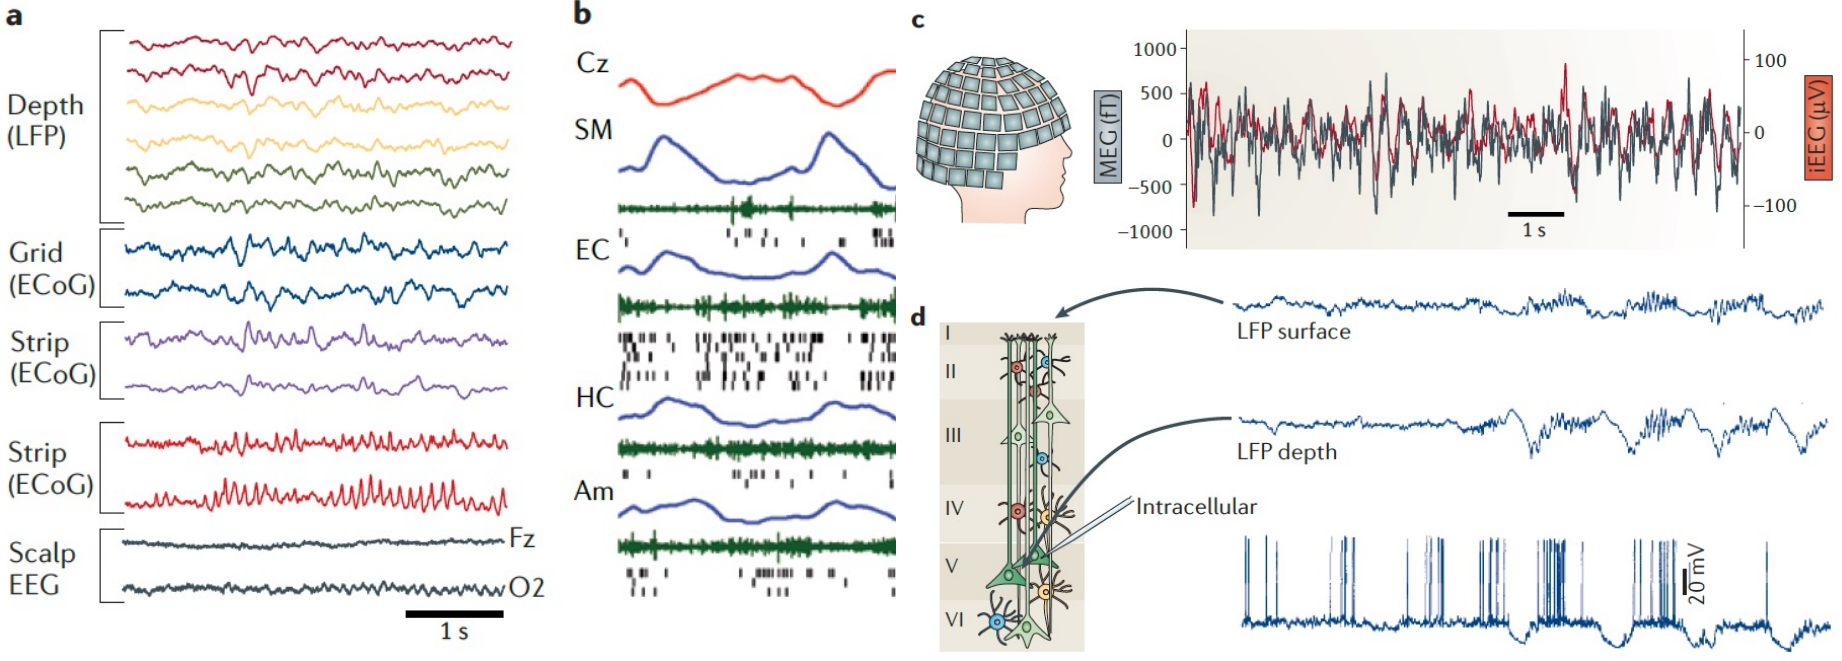
\includegraphics[scale=0.42]{9_1}
    \centering
\end{figure}
\subsubsection{LFP Recording Techniques}
The first attempt at recording LFPs was made in 1927, when Hans Berger recorded alpha
oscillations for the first time, which appear with closed eyes and disappear when
they are open. This is related to the fact that when the eyes are closed, all neurons
in V1 fire and respond to the same stimulus, while when the eyes are open, different
parts of V1 respond to different properties of the stimuli. When all the neurons are
synchronized, the local field potential will be larger and it will be easier to
record also from far away. The \textit{in vivo} Local Field Potential signal is mainly
recorded by exploiting two techniques:
\begin{itemize}
    \item \textbf{Electrocorticography (ECoG):} subdural grids are placed directly on
          the top of the cortex, under the dura mater, resulting in a significantly
          invasive implant.
    \item \textbf{Stereo Electroencephalography (SEEG):} linear multi-electrode shafts
          are directly implanted into the grey matter, thus the invasiveness is reduced,
          as only small holes on the skull are necessary to insert the long linear electrodes.
\end{itemize}
These systems live roughly in the same range as EEG, but their signals are one order of
magnitude larger, because their electrodes are more in contact with the neural population
that is generating the activity and the signals do not have to travel across the layers of
the head (and so there is no low-pass filtering).
\subsubsection{LFP Signal Components}
In order to understand the meaning of the Local Field Potential, it is fundamental to
focus on which are the factors that contribute to generate it. The extracellular
field is a superimposition of:
\begin{itemize}
    \item Any excitable membrane (such as axons), always trying to balance the inner
          and outer ions concentrations, generating electrical currents. The amount
          of current that is produced depends on the size of the cell and on the type
          of input that it has.
    \item Synaptic activity between cells, generating the largest extracellular
          currents.
    \item Fast action potentials, where Na\({}^+\) ions contributes to high frequency
          activity.
    \item Calcium spikes, recorded by exploiting calcium imaging techniques.
    \item Intrinsic currents and resonances, giving birth to membrane responses.
    \item Spikes after hyperpolarization.
    \item \dots
\end{itemize}
In general, it can be stated that the surrounding activity of neurons highly affects
the LFP by influencing the transmembrane potential of cells.
\begin{figure}[H]
    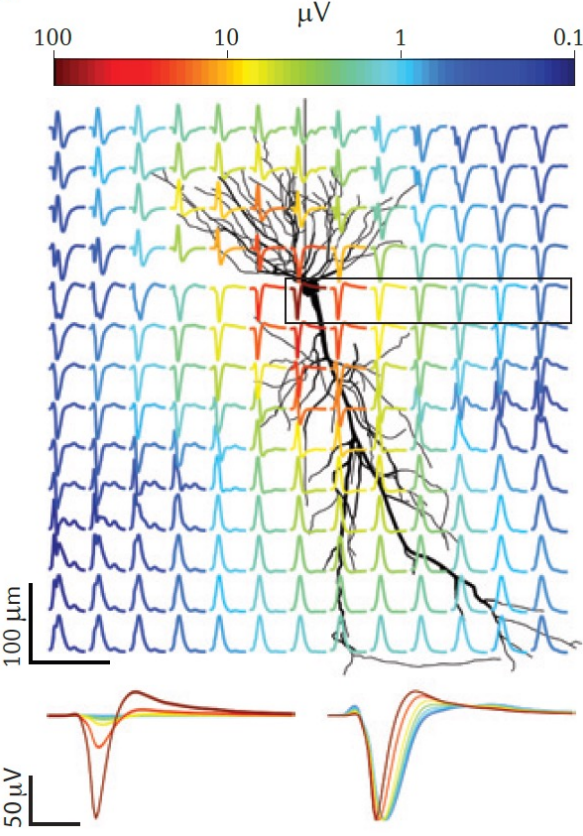
\includegraphics[scale=0.42]{9_2}
    \centering
\end{figure}
\subsubsection{Neural Architecture and Geometry}
Also the neuronal \textbf{geometry} as well as the \textbf{architecture} have a huge
impact on the recorded LFP signal. In particular, neurons can be roughly divided into
two main classes: linear and spherical (often called stellate). The shape of a neuron
highly influences the way the electrical signal travels and propagates in the
extracellular field.
\begin{itemize}
    \item Much of the signal taken into account comes from \textbf{pyramidal neurons},
          cells that belong to the linear class, characterized by a very specific
          geometry and orientation, able to create aligned electrical dipoles, which
          generate very strong electrical field potentials.
    \item On the contrary, \textbf{spherical neurons} tend to emanate dendrites of
          approximately equal size in all directions, implying almost no separation
          between sink and source, with a small contribution to the overall electrical
          field, as signals cancel each other out.
\end{itemize}
This is even more complex when the whole structure of cortical columns is considered,
with their different layers containing multiple types and densities of cells.
\begin{figure}[H]
    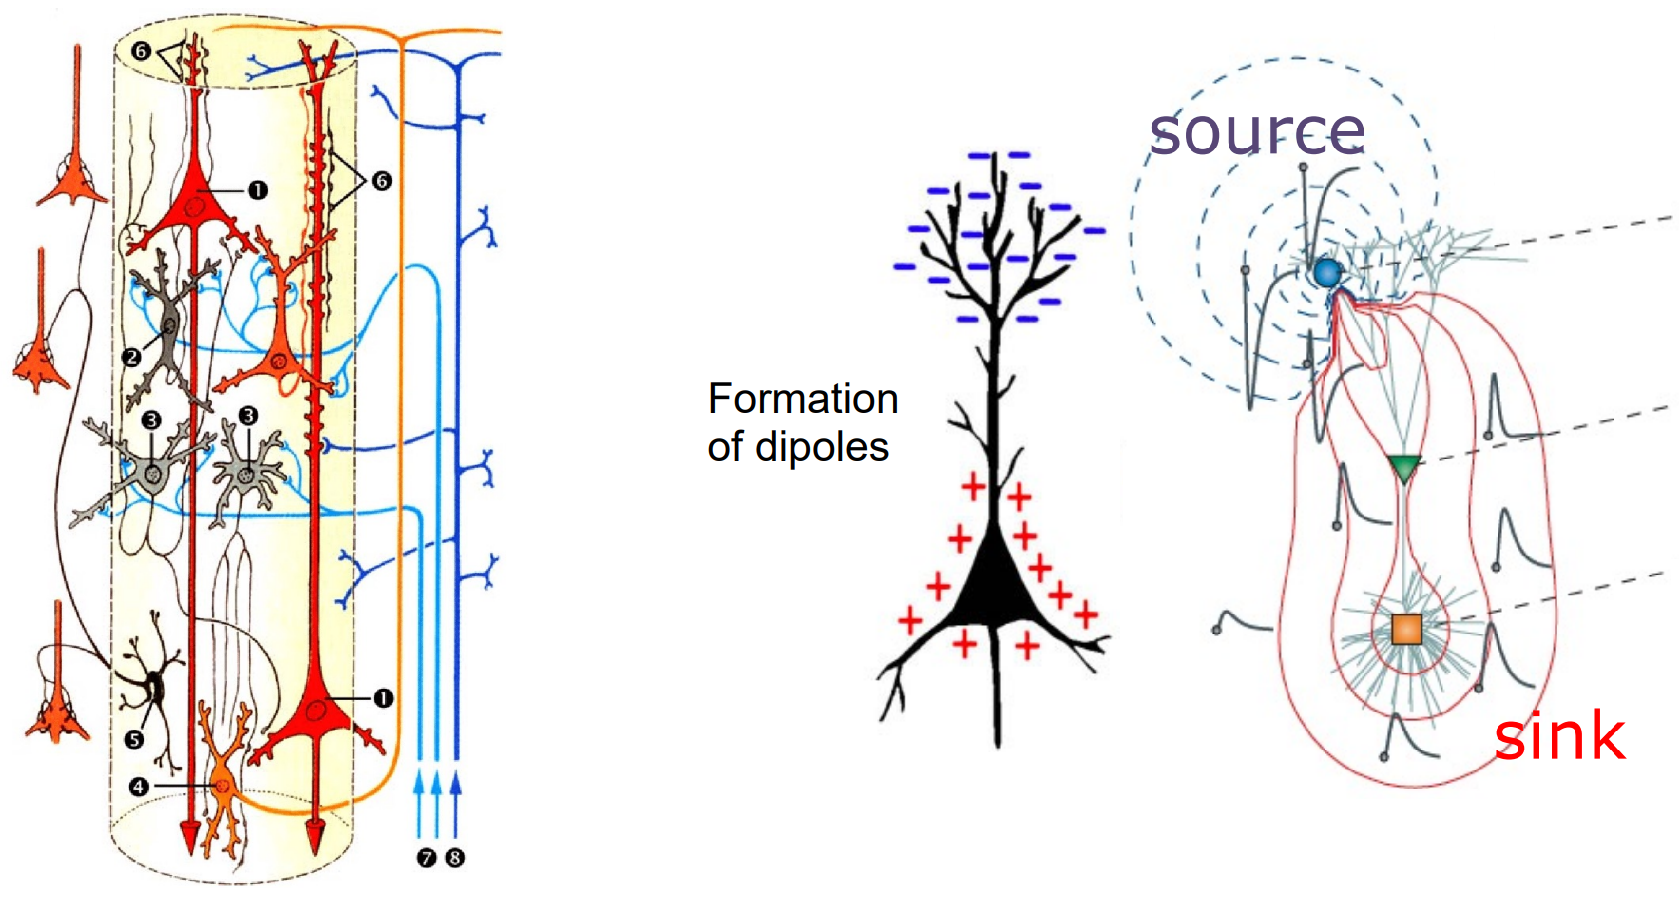
\includegraphics[scale=0.35]{9_3}
    \centering
\end{figure}
A further factor affecting the LFP signal is the \textit{temporal scaling}. A temporal
superimposition of a large number of activated neurons will increase the LFP signal:
this phenomenon is known as \textbf{synchronization}. The so-called \textit{Beta rhythm},
for instance, is a peculiar type of synchronization that lies between \(13\) and
\(30\,Hz\). It mostly occurs in reaching and motion tasks, but this synchronization
is suppressed as soon as the reaching movement is completed. Another important feature
of temporal scaling is the \(\frac{1}{f^{\alpha}}\) frequency decay: the amplitude of
the signal exhibits a power-law decay towards high frequencies and this may be
partially explained by the low-pass filtering performed by dendrites and the
conductive media that the electrical field has to travel into.

\subsection{The Forward Problem}
By assuming a homogeneous and isotropic conductivity, it is possible to easily
solve the so-called \textit{forward problem} by exploiting the Maxwell's equations.
The \textit{forward problem} consists in reconstructing the measured eletrical field
- i.e., the LFP - by knowning the sources which generated it. Unluckily, the
brain conductivity is neither homogeneous nor isotropic, and this generates several
problems when studying how the eletrical signal propagates through the neural tissue.
This phenomenon is thus denominated \textbf{volume conduction}. Generally, when
analyzing a neural signal, it is believed that coherent activity reflects functionally
relevant processing; however, volume conductivity represents a significant issue, as
it tends to amplify this, leading to an overestimation of the coherent activity
in brain.\\
More in detail, the \textit{forward problem} indicates the modelling of the system
responsible for the generation of a given recorded signal. It is opposed to the
\textit{inverse problem}, consisting in sources localization. A possible approach
to the \textit{forward problem} is by exploiting compartmental models, then
properly tuning the model parameters. Although this approach looks promising,
it is computationally costly. On the other hand, single-compartment models
are too simplistic to properly describe the structure of a neuron.\\
When trying to address the \textit{forward problem} it is important to recall
that the synaptic connectivity highly affects the LFP. On one side, it
determines the spike train statistics (the so-called temporal coding), creating
correlation patterns for the synaptic inputs and, on the other side, the spatial
distribution of synapses highly affects how inputs are translated into LFP.
To sum up, it is not just a single neuron geometry that determines the LFP
dynamics, but also the network spatial distribution: at the micro and meso
scales the structure of the network plays a crucial role in determining
the function.

\subsection{Functional Decomposition}
The Local Field Potential, as well as other signals such as EEG and MEG ones,
is usually decomposed into several frequency bands thanks to filtering.
These bands are often called Berger Bands. They are far from being accurate
between different subjects and even within the same subject in
different time instants. \\
Usually, three main groups are determined by looking at the correlation between
two signals as a function of their frequency:
\begin{itemize}
    \item Slow rhythms with a high oscillatory activity: from \(0\,Hz\) to \(50\,Hz\)
    \item Gamma oscillations mediated by rhythmic inhibition: from \(50\,Hz\)
          to \(100\,Hz\)
    \item High gamma activity, reflecting the Multi Unit Activity (MUA) close
          to the electrode, proportional to the real spiking activity:
          from \(100\,Hz\) to \(150\,Hz\)
\end{itemize}
\begin{figure}[H]
    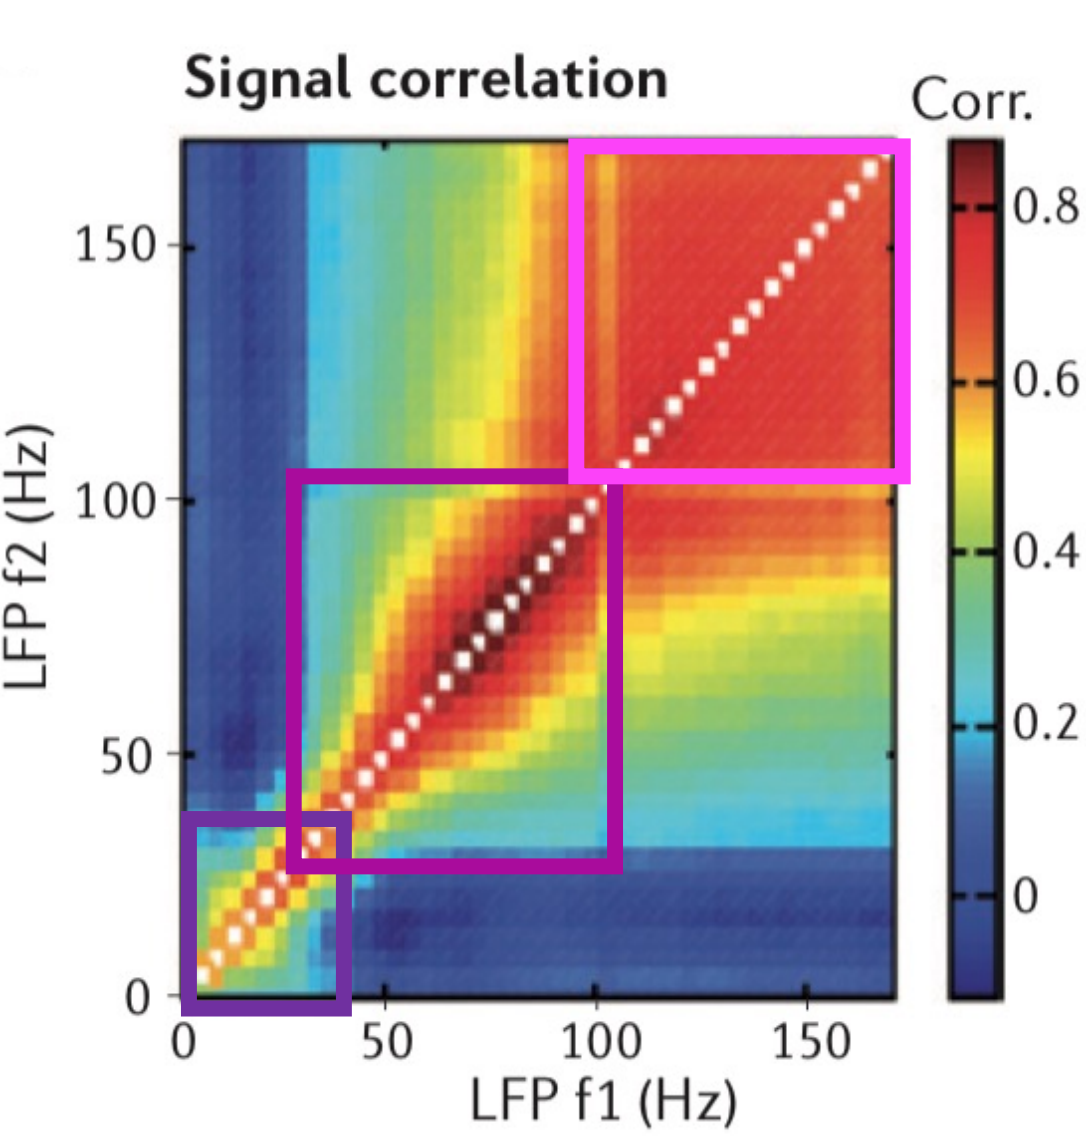
\includegraphics[scale=0.25]{9_4}
    \centering
\end{figure}

\subsection{Spikes Contribution to LFP}
A very important part of LFP is given by the so-called \textbf{high gamma range} or
\textbf{ripple range}. The signals belonging to this interval are quite fast
(above \(100\,Hz\)), hence they cannot be easily recorded with scalp electrodes, but
require deep ones. They are pretty much important because they are the direct
correlate of the multi-unit activity coming from an extracellular electrode. Hence,
they are basically the only way to record some byproducts of the real spiking activity
in humans.\\
Therefore, it is possible to look at the spiking activity of specific brain regions by
filtering the recorded signals in the frequency range above \(100-120\,Hz\): the LFPs
provide an indirect measure of the spike activity of the neuron ensemble.
